\section{Problem Formulation and Verifier Taxonomy}
\label{sec:setup}

We study verification as a relationship between a claim, an evidence substrate,
and an access regime.  The same signal can be persuasive in one regime and
unusable in another.  A provider-side event trace may support a cooperative
audit, while copied final text may not preserve the same witness.  This section
defines the verifier axes used throughout the paper.

\begin{definition}[Verification substrate]
A verification substrate is the object that carries or preserves evidence for a
claim.  Examples include platform metadata, protocol transcripts, proof
objects, provider-side token-event traces, model-state access, and natural
final text.
\end{definition}

\paragraph{Verifier axes.}
We use six axes to avoid conflating different verification regimes.
\begin{description}
\item[Public.] A third party can inspect the evidence object or run the stated
test without private platform access.
\item[Deterministic.] The test recovers a codeword, proof, exact witness, or
precommitted object rather than only a distributional correlation.
\item[Portable.] The evidence travels with ordinary copies or redistribution of
the output.
\item[Natural-output-native.] The evidence is not an obvious Step label, fixed
slot, public watermark literal, external certificate, or visible proof object.
\item[Non-cooperative.] The suspect need not provide weights, metadata, logs,
special API behavior, or a trace bundle.
\item[Hard to spoof.] Public feedback does not cheaply let an attacker create
accepted source-mismatch examples.
\end{description}

No current artifact in this paper satisfies all six axes simultaneously.  The
supported diagnostic result is trace-bound and cooperative: an authorized
verifier has access to provider-side first-divergence token-event traces.  The
unsupported target is stronger: a public final-text-only method that is
deterministic, portable, non-cooperative, natural-output-native, and hard to
spoof.  That target remains unsupported by the current artifacts.

\begin{principle}[Substrate displacement]
\label{prin:substrate-displacement}
Moving evidence from ordinary final text to a stronger substrate can increase
determinism, auditability, or spoof resistance only for access regimes in
which that stronger substrate is available.  A result established over a
metadata, protocol, proof, trace, or model-state substrate therefore does not
automatically transfer to a copied-final-text regime.
\end{principle}

Principle~\ref{prin:substrate-displacement} is a scope rule rather than an
impossibility theorem.  It is the reason we separate trace-bound diagnostics
from public final-text predicates throughout the manuscript.  Trace-bound
codeword recovery can demonstrate provider-side event controllability, but it
does not become a public final-text claim when the trace is absent.

\begin{table}[t]
\centering
\scriptsize
\setlength{\tabcolsep}{3pt}
\begin{tabular}{p{0.17\linewidth}p{0.12\linewidth}p{0.12\linewidth}p{0.12\linewidth}p{0.12\linewidth}p{0.25\linewidth}}
\toprule
Substrate & Public & Deterministic & Portable & Non-coop. & Current role \\
\midrule
Metadata & Sometimes & Sometimes & Fragile & Sometimes & Strong only if preserved \\
Protocol transcript & Usually & Often & No & No & Strong under participation \\
Proof object & Yes & Yes & Conditional & Conditional & Requires a statement and proof \\
Provider trace & No & Yes & No & No & Supported cooperative diagnostic \\
Model state & No & Often & No & No & White-box or cooperative evidence \\
Natural final text & Yes & Not shown & Yes & Yes & Current public substrate fails codeword recovery \\
\bottomrule
\end{tabular}
\caption{Verification substrates differ in which properties they can support.
The table is a taxonomy, not a ranking.  Current results support the provider
trace row under cooperative event access; they are not public text-only
verification success.}
\label{tab:substrate-taxonomy}
\end{table}

\begin{figure}[t]
\centering
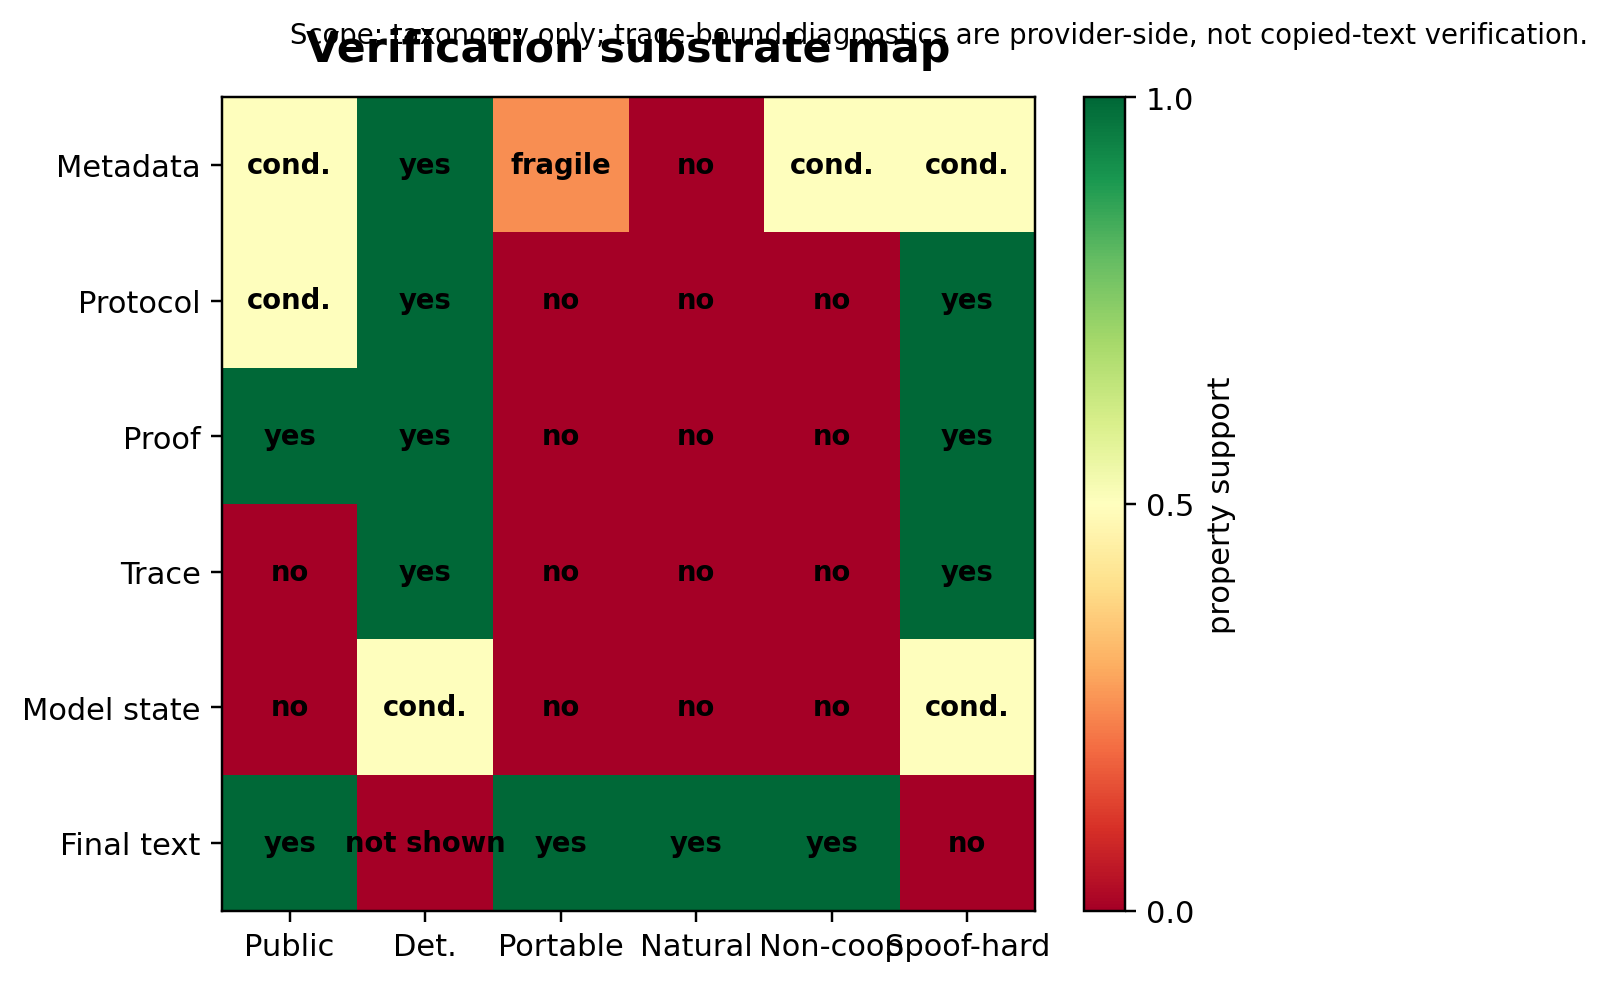
\includegraphics[width=\linewidth]{figures/figure_1_verification_substrate_map.png}
\caption{Verification substrate map.  The map summarizes which properties
different substrates can support.  It is a taxonomy and does not claim a
universal impossibility theorem; it is not public text-only verification
success and not an ownership proof.}
\label{fig:substrate-map}
\end{figure}

\paragraph{Threat model.}
The public final-text setting assumes an observer sees only the generated text.
The observer does not receive the model weights, hidden states, logits,
provider logs, trace bundles, or cryptographic signatures.  The attacker may
query a public predicate, search over source-mismatch examples, apply simple
rewrites, learn a surrogate ranker from public feedback, and optimize text
against the predicate.  The attacker is not assumed to know a private provider
key for the trace-bound diagnostic.

\paragraph{Source-mismatch examples.}
A source-mismatch example is a row produced by a source that should not satisfy
the protected claim, such as raw, task-only, wrong-key, or wrong-payload text.
If a public predicate accepts such a row, that acceptance is spoofing evidence
against the predicate.  It is not protected success, not codeword recovery, not
natural evidence success, and not an ownership proof.

\paragraph{Current claim boundary.}
The supported claim is limited to the following statement: reviewed Qwen and
Llama trace-bound diagnostics show provider-side event controllability under
authorized trace access, while public final-text predicates in the current
artifacts recover zero codeword blocks and are vulnerable to source-mismatch
optimization.  The paper does not claim public text-only verification success,
cryptographic provenance, signed trace provenance, sanitizer robustness,
payload-diversity evidence, or model-family general verification.
